% Options for packages loaded elsewhere
\PassOptionsToPackage{unicode}{hyperref}
\PassOptionsToPackage{hyphens}{url}
\PassOptionsToPackage{dvipsnames,svgnames,x11names}{xcolor}
%
\documentclass[
  letterpaper,
  DIV=11,
  numbers=noendperiod]{scrartcl}

\usepackage{amsmath,amssymb}
\usepackage{iftex}
\ifPDFTeX
  \usepackage[T1]{fontenc}
  \usepackage[utf8]{inputenc}
  \usepackage{textcomp} % provide euro and other symbols
\else % if luatex or xetex
  \usepackage{unicode-math}
  \defaultfontfeatures{Scale=MatchLowercase}
  \defaultfontfeatures[\rmfamily]{Ligatures=TeX,Scale=1}
\fi
\usepackage{lmodern}
\ifPDFTeX\else  
    % xetex/luatex font selection
\fi
% Use upquote if available, for straight quotes in verbatim environments
\IfFileExists{upquote.sty}{\usepackage{upquote}}{}
\IfFileExists{microtype.sty}{% use microtype if available
  \usepackage[]{microtype}
  \UseMicrotypeSet[protrusion]{basicmath} % disable protrusion for tt fonts
}{}
\makeatletter
\@ifundefined{KOMAClassName}{% if non-KOMA class
  \IfFileExists{parskip.sty}{%
    \usepackage{parskip}
  }{% else
    \setlength{\parindent}{0pt}
    \setlength{\parskip}{6pt plus 2pt minus 1pt}}
}{% if KOMA class
  \KOMAoptions{parskip=half}}
\makeatother
\usepackage{xcolor}
\setlength{\emergencystretch}{3em} % prevent overfull lines
\setcounter{secnumdepth}{-\maxdimen} % remove section numbering
% Make \paragraph and \subparagraph free-standing
\ifx\paragraph\undefined\else
  \let\oldparagraph\paragraph
  \renewcommand{\paragraph}[1]{\oldparagraph{#1}\mbox{}}
\fi
\ifx\subparagraph\undefined\else
  \let\oldsubparagraph\subparagraph
  \renewcommand{\subparagraph}[1]{\oldsubparagraph{#1}\mbox{}}
\fi


\providecommand{\tightlist}{%
  \setlength{\itemsep}{0pt}\setlength{\parskip}{0pt}}\usepackage{longtable,booktabs,array}
\usepackage{calc} % for calculating minipage widths
% Correct order of tables after \paragraph or \subparagraph
\usepackage{etoolbox}
\makeatletter
\patchcmd\longtable{\par}{\if@noskipsec\mbox{}\fi\par}{}{}
\makeatother
% Allow footnotes in longtable head/foot
\IfFileExists{footnotehyper.sty}{\usepackage{footnotehyper}}{\usepackage{footnote}}
\makesavenoteenv{longtable}
\usepackage{graphicx}
\makeatletter
\def\maxwidth{\ifdim\Gin@nat@width>\linewidth\linewidth\else\Gin@nat@width\fi}
\def\maxheight{\ifdim\Gin@nat@height>\textheight\textheight\else\Gin@nat@height\fi}
\makeatother
% Scale images if necessary, so that they will not overflow the page
% margins by default, and it is still possible to overwrite the defaults
% using explicit options in \includegraphics[width, height, ...]{}
\setkeys{Gin}{width=\maxwidth,height=\maxheight,keepaspectratio}
% Set default figure placement to htbp
\makeatletter
\def\fps@figure{htbp}
\makeatother

\KOMAoption{captions}{tableheading}
\makeatletter
\@ifpackageloaded{caption}{}{\usepackage{caption}}
\AtBeginDocument{%
\ifdefined\contentsname
  \renewcommand*\contentsname{Table of contents}
\else
  \newcommand\contentsname{Table of contents}
\fi
\ifdefined\listfigurename
  \renewcommand*\listfigurename{List of Figures}
\else
  \newcommand\listfigurename{List of Figures}
\fi
\ifdefined\listtablename
  \renewcommand*\listtablename{List of Tables}
\else
  \newcommand\listtablename{List of Tables}
\fi
\ifdefined\figurename
  \renewcommand*\figurename{Figure}
\else
  \newcommand\figurename{Figure}
\fi
\ifdefined\tablename
  \renewcommand*\tablename{Table}
\else
  \newcommand\tablename{Table}
\fi
}
\@ifpackageloaded{float}{}{\usepackage{float}}
\floatstyle{ruled}
\@ifundefined{c@chapter}{\newfloat{codelisting}{h}{lop}}{\newfloat{codelisting}{h}{lop}[chapter]}
\floatname{codelisting}{Listing}
\newcommand*\listoflistings{\listof{codelisting}{List of Listings}}
\makeatother
\makeatletter
\makeatother
\makeatletter
\@ifpackageloaded{caption}{}{\usepackage{caption}}
\@ifpackageloaded{subcaption}{}{\usepackage{subcaption}}
\makeatother
\ifLuaTeX
  \usepackage{selnolig}  % disable illegal ligatures
\fi
\IfFileExists{bookmark.sty}{\usepackage{bookmark}}{\usepackage{hyperref}}
\IfFileExists{xurl.sty}{\usepackage{xurl}}{} % add URL line breaks if available
\urlstyle{same} % disable monospaced font for URLs
\hypersetup{
  pdftitle={The End of Decision Theory},
  pdfauthor={Brian Weatherson},
  colorlinks=true,
  linkcolor={blue},
  filecolor={Maroon},
  citecolor={Blue},
  urlcolor={Blue},
  pdfcreator={LaTeX via pandoc}}

\title{The End of Decision Theory}
\author{Brian Weatherson}
\date{}

\begin{document}
\maketitle

\section{What is Decision Theory a Theory
Of?}\label{what-is-decision-theory-a-theory-of}

If you're reading a journal like this, you're probably familiar with
seeing papers defending this or that decision theory. Familiar decision
theories include:

\begin{itemize}
\tightlist
\item
  Causal Decision Theory {[}@GibbardHarper1979; @Lewis1980; @Skyrms1990;
  @Joyce199x{]};
\item
  Evidential Decision Theory {[}@Ahmed2013{]};
\item
  Benchmark theory {[}@Wedgwood2013{]};
\item
  Risk-Weighted theory {[}@BuchakRiskRationality{]};
\item
  Tournament Decision Theory {[}@Podgorski2020{]}; and
\item
  Functional Decision Theory {[}@LevinsteinSoares2020{]}
\end{itemize}

Other theories haven't had snappy `isms' applied to them, such as the
non-standard version of Causal Decision Theory that Dmitri @Gallow2020
defends, or the pluralist decision theory that Jack @Spencer2021
defends, or the broadly ratificationist theory that Melissa @Fuscond
defends

This paper isn't going to take sides between these nine or more
theories.\footnote{The arguments here are intended to support a theory
  like Fusco's, but in a fairly roundabout way, but the connection
  between what I say here and Fusco's theory would take a paper as long
  as this one to set out.} Rather it is going to ask a prior pair of
questions.

\begin{enumerate}
\def\labelenumi{\arabic{enumi}.}
\tightlist
\item
  If these are the possible answers, what is the question? That is, what
  is the question to which decision theories are possible answers?
\item
  Why is that an interesting question? What do we gain by answering it?
\end{enumerate}

On 1, I will argue that decision theories are answers to a question
about what an ideal decider would do. The `ideal' here is like the
`ideal' in a scientific idealisation, not the ideal in something like an
ideal advisor moral theory. That is, the ideal decider is an
idealisation in the sense of being simple, not in the sense of being
perfect. The ideal decision maker is ideal in the same way that the
point-masses in the ideal gas model are ideal; they are (relatively)
simple to work with. The main opponent I have in mind is someone who
says that in some sense decision theory tells us what decisions we
should make.

On 2, I will argue that the point of asking this question is that these
idealisations play important roles in explanatorily useful models of
social interactions, such as the model of the used car market that Georg
@Akerlof1970 described. Here, the main opponent I have in mind is
someone who says that decision theory is useful because it helps us make
better decisions.

There is another pair of answers to this question which is interesting,
but which I won't have a lot to say about here. David Lewis said that
decision theory was in the business of setting out a key part of the
notion of rationality that is constitutive of having mental states. It
is important on this view that we get decision theory right because the
details might matter to the right theory of mental content. I think the
arguments I give for my preferred view provide some reasons to be
sceptical of this view, but they are far from conclusive reasons against
it. My main purpose is to argue against the claim that decision theory
says anything about what we should do, or that it provides us with
advice.\footnote{Lewis's views about the role of decision theory are set
  out in \ldots{} . In a letter to \ldots{} he says that the advisory
  role of decision theory is one that he would ``downplay'', but he
  still seems to make it more central than I would do.}

The nine theories I mentioned above disagree about a lot of things. In
philosophy we typically spend our time looking at cases where theories
agree. Not here! I will focus almost exclusively on two cases where
those nine theories all say the same thing. I'll assume that whatever
question they are asking, the correct answer to it in those two cases
must agree with all nine theories. That will be enough to defend the
view I want to defend, which is that a decision theory is correct iff is
true in the right kind of idealisation.

\section{Three Cases}\label{three-cases}

\subsection{Betting}\label{betting}

Chooser has \$110, and is in a sports betting shop. There is a
basketball game about to start, between two teams they know to be
equally matched. Chooser has three options: bet the \$110 on Home, bet
it on Away, keep money. If they bet and are right, they win \$100 (plus
get the money back they bet), if they are wrong, they lose the money.
Given standard assumptions about how much Chooser likes money, all the
decision theories I'm discussing say Chooser should not bet.

From this it follows that decision theory is not in the business of
answering this question: \emph{What action will produce the best
outcome?}. We know, and so does Chooser, that the action that produces
the best outcome is to bet on the winning team. Keeping their money in
their pocket is the only action they know will be sub-optimal. And it's
what decision theory says to do.

This is to say, decision theory is not axiology. It's not a theory of
evaluating outcomes, and saying which is best. Axiology is a very
important part of philosophy, but it's not what decision theorists are
up to.

So far this will probably strike you, dear reader, as obvious. But
there's another step, that I think will strike some people as nearly as
obvious, that I'm at pains to resist. Some might say that decision
theorists don't tell Chooser to bet on the winner because this is lousy
advice. Chooser can't bet on the winner, at least not as such. That,
I'll argue, would be a misstep. Decision theorists do not restrict
themselves to answers that can be practically carried out.

\subsection{Salesman}\label{salesman}

We'll focus on a version of what Julia @Robinson1949 called the
traveling salesman problem. Given some points on a map, find the
shortest path through them. We'll focus on the 257 cities shown on the
map in Figure~\ref{fig-map}.

\begin{verbatim}
Loading required package: tidyverse
\end{verbatim}

\begin{verbatim}
-- Attaching core tidyverse packages ------------------------ tidyverse 2.0.0 --
v dplyr     1.1.4     v readr     2.1.5
v forcats   1.0.0     v stringr   1.5.1
v ggplot2   3.5.1     v tibble    3.2.1
v lubridate 1.9.3     v tidyr     1.3.1
v purrr     1.0.2     
-- Conflicts ------------------------------------------ tidyverse_conflicts() --
x dplyr::filter() masks stats::filter()
x dplyr::lag()    masks stats::lag()
i Use the conflicted package (<http://conflicted.r-lib.org/>) to force all conflicts to become errors
Loading required package: TSP

Loading required package: maps


Attaching package: 'maps'


The following object is masked from 'package:purrr':

    map


Loading required package: grid
\end{verbatim}

\begin{verbatim}
Warning: A numeric `legend.position` argument in `theme()` was deprecated in ggplot2
3.5.0.
i Please use the `legend.position.inside` argument of `theme()` instead.
\end{verbatim}

\begin{figure}

\centering{

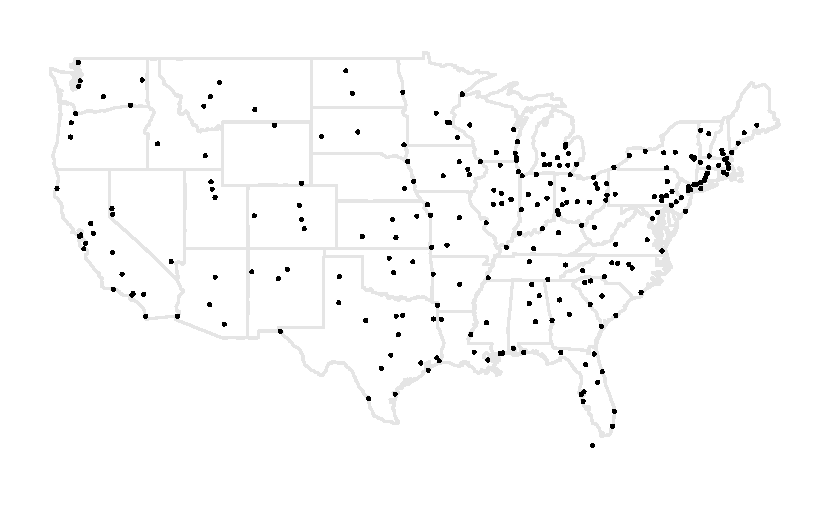
\includegraphics{teodt2024_paper_files/figure-pdf/fig-map-1.pdf}

}

\caption{\label{fig-map}257 American cites; we'll try to find the
shortest path through them.}

\end{figure}%

The task is to find the shortest path through those 257
cities.\footnote{Include citation as to where I got the map, and the
  packages used in this, and to where I learned some of this stuff about
  TS problems.}

All nine of the decision theories I mentioned, and as far as I know
every competitor to them in the philosophical literature, say the thing
to do here is to draw whichever of the 256! possible paths is shortest.
That is not particularly helpful advice. Unless you know a lot about
problems like this, you can't draw the shortest path through the map.
And least, you can't draw it as such. You can't draw it in the way that
you can't enter the correct code on a locked phone
{[}@MandlekernEtAl2017{]}.

One of the striking things about this puzzle is that it turns out there
are some helpful things that can be said. One helpful bit of advice to
someone trying to solve a problem like this is to use a Farthest
Insertion Algorithm. Insertion algorithms say to start with a random
city, then add cities to the path one at a time, at each time finding
the point to insert the city into the existing path that adds the least
distance. The Farthest Insertion Algorithm says that the city added at
each stage is the one farthest from the existing path. Insertion
algorithms in general produce pretty good paths in a very short amount
of time - at least on normal computers. And the Farthest Insertion
Algorithm is, most of the time, the best Insertion Algorithm to use.
Figure~\ref{fig-farthest} shows the result of one output of this
algorithm.\footnote{The algorithm is silent on which city you start
  with, and usually chooses this randomly.}

\begin{figure}

\centering{

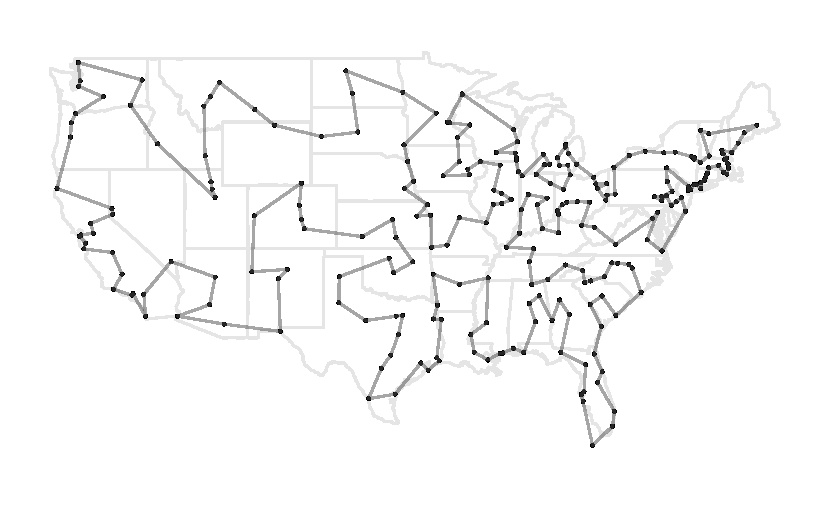
\includegraphics{teodt2024_paper_files/figure-pdf/fig-farthest-1.pdf}

}

\caption{\label{fig-farthest}An output of the Farthest Insertion
Algorithm, with a length of 21197 miles.}

\end{figure}%

The path in Figure~\ref{fig-farthest} is not bad, but with only a bit of
extra computational work, one can do better. A fairly simple
optimisation algorithm takes a map as input, and then deletes pairs of
edges at a time, and finds the shortest path of all possible paths with
all but those two edges. The process continues until no improvements can
be made by deleting two edges at a time, at which point you've found a
somewhat resilient local minimum. Figure~\ref{fig-two_opt} is the output
from applying this strategy to the path in Figure~\ref{fig-farthest}.

\begin{verbatim}
[1] FALSE
\end{verbatim}

\begin{figure}

\centering{

\includegraphics{teodt2024_paper_files/figure-pdf/fig-two_opt-1.pdf}

}

\caption{\label{fig-two\_opt}An output of the Farthest Insertion
Algorithm, with a length of 21197 miles.}

\end{figure}%

This optimisation tends to produce paths that look a lot like the
original, but are somewhat shorter. For most practical purposes, the
best advice you could give someone faced with a problem like this is to
use a Farthest Insertion Algorithm, then optimise it in this way. Or, if
they have a bit more time, they could do this a dozen or so times, and
see if different starting cities led to slightly shorter paths.

While this is good advice, and indeed it's what most people should do,
it's not typically what is optimal to do. For that reason, it's not what
our nine decision theories would say to do. If one had unlimited and
free computing power available, hacks like these would be pointless. One
would simply look at all the possible paths, and see which was shortest.
I do not have free, unlimited computing power, so I didn't do this.
Using some black box algorithms I did not particularly understand, I was
able to find a shorter path, however. It took some time, both of mine
and my computer's, and for most purposes it would not have been worth
the hassle of finding it. Still, just to show it exists, I've plotted it
as Figure~\ref{fig-best}.

\begin{verbatim}
[1] TRUE
\end{verbatim}

\begin{figure}

\centering{

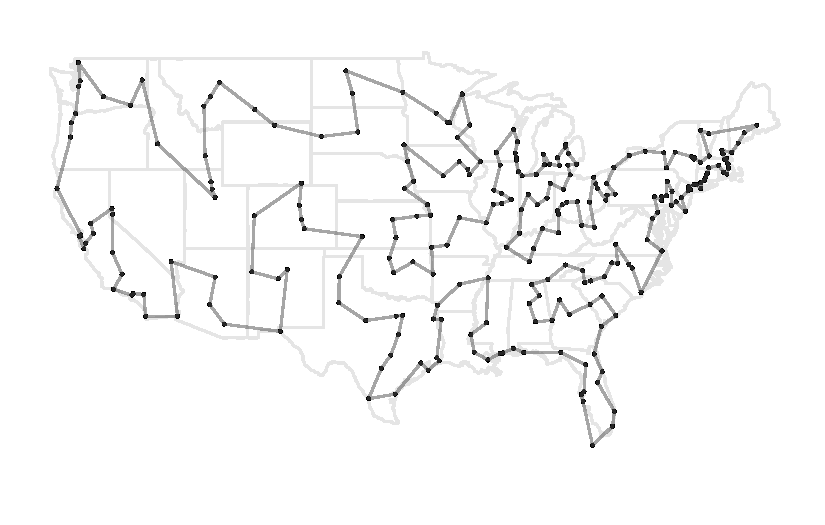
\includegraphics{teodt2024_paper_files/figure-pdf/fig-best-1.pdf}

}

\caption{\label{fig-best}An output of the Farthest Insertion Algorithm,
with a length of 21197 miles.}

\end{figure}%

I'm not sure if Figure~\ref{fig-best} is as short as possible, but I
couldn't find a shorter one. Still, unless those 200 miles really make a
difference, it wouldn't have been worth the trouble it took to find this
map.

\subsection{The Two Cases}\label{the-two-cases}

Let's summarise these two cases in a table.

\begin{longtable}[]{@{}lcc@{}}
\toprule\noalign{}
& Betting & Salesman \\
\midrule\noalign{}
\endhead
\bottomrule\noalign{}
\endlastfoot
Best outcome & Bet on winner & Shortest path \\
Decision theory & Pass & Shortest path \\
Best advice & Pass & Learn algorithms \\
\end{longtable}

The first row says which action would produce the best outcome in the
two cases. The third row says what advice one ought give someone who had
to choose in the two cases. And the middle row says what all the
decision theories say about the two cases. Notably, it agrees with
neither the first nor third row. Decision theory is neither in the
business of saying what will produce the best result, nor with giving
the most useful advice. So what is it doing?

\section{Decision Theory as
Idealisation}\label{decision-theory-as-idealisation}

Imagine a version of Chooser with, as Rousseau might have put it, their
knowledge as it is, and their computational powers as they might be.
That is, a version of Chooser who has unlimited, and free, computational
powers, but no more knowledge of the world than the actually have - save
what they learn by performing deductions from their existing knowledge.

Decision theories describe what that version of Chooser would do in the
problem that Chooser is facing. In the betting case, adding unlimited
computing power doesn't tell you who is going to win the game. So that
version of Chooser will still avoid betting. But in the Salesman case,
adding unlimited computing power is enough to solve the problem. They
don't even have to use any fancy techniques. To find the shortest path,
all it takes is finding the length of each path, and sorting the
results. The first requires nothing more that addition; at least if, as
was the case here, we provided the computer with the distances between
any pairs of cities as input. The second just requires being able to do
a bubble sort, which is technically extremely simple. To be sure, doing
all these additions, then doing a bubble sort on the results, will take
longer than most human lives on the kinds of computers most people have
available to them. But a version of Chooser with unlimited, free,
computational power will do these computations no problem at all.

If we say that

\subsection{Technical Detour}\label{technical-detour}

Most philosophical decision theory concerns decisions under uncertainty,
not decisions like Salesman that are made under certainty.

\begin{itemize}
\tightlist
\item
  But the structure is still the same.
\end{itemize}

\subsection{Technical Detour}\label{technical-detour-1}

They say that for each option, you should loop through the possible
states of the world, in each case multiplying something (usually a
probability) by something else (usually a utility), and then summing the
results. Then you choose the maximum.

\begin{itemize}
\tightlist
\item
  That's exactly the same technical task as solving Salesman by brute
  force.\footnote{Actually one step harder because of the
    multiplication, but otherwise the same.}
\end{itemize}

\subsection{Summary}\label{summary}

Decision theory describes what a particular kind of idealised agent
\textbf{will} do.

\begin{itemize}
\tightlist
\item
  I've bolded \textbf{will} because it's going to turn out that's the
  important modal to use here; as opposed to \emph{should}.
\item
  If there is any normativity here, it's in the \textbf{idealised} part
  of that sentence, not the modal.
\end{itemize}

\section{Idealisations as Life Goals}\label{idealisations-as-life-goals}

\subsection{A Modest Proposal}\label{a-modest-proposal}

Decision theory is relevant to how we should act because:

\begin{enumerate}
\def\labelenumi{\arabic{enumi}.}
\tightlist
\item
  It tells us that idealised people do use decision theory, and
\item
  We should try to be like idealised people.
\end{enumerate}

\begin{enumerate}
\def\labelenumi{\Alph{enumi}.}
\setcounter{enumi}{2}
\tightlist
\item
  We should try to use decision theory.
\end{enumerate}

\begin{center}\rule{0.5\linewidth}{0.5pt}\end{center}

\begin{figure}[H]

{\centering 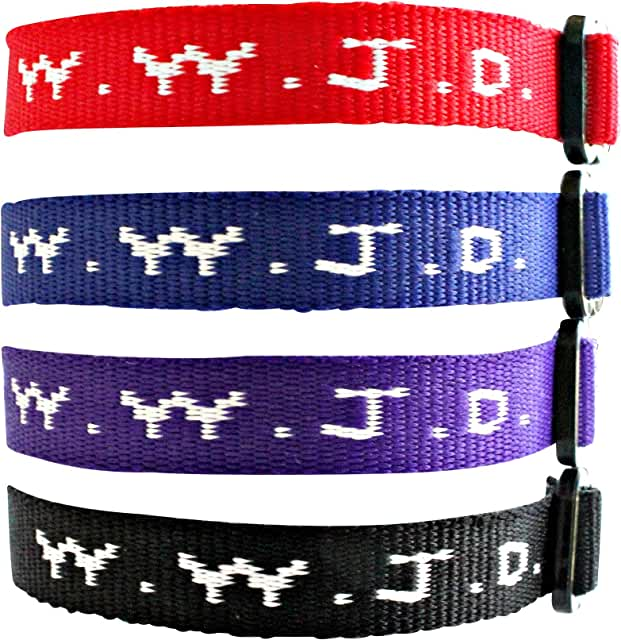
\includegraphics{bracelet.jpg}

}

\caption{I think this stands for What Would Jeffrey Do?}

\end{figure}%

\subsection{First Objection - Knowing the
Inputs}\label{first-objection---knowing-the-inputs}

To use decision theory as a guide to action, I need to know the utility
of the possible states.

\begin{itemize}
\tightlist
\item
  Knowing ordering isn't enough, need cardinality of each utility.
\item
  I can only ever tell that the utility of A is half way between that of
  B and C by thinking about whether A is better or worse to take than a
  50/50 bet on B or C.
\item
  I need to make decisions to get the inputs to decision theory.
\item
  And I think this is the usual case.
\end{itemize}

\subsection{Second Objection - The General Theory of the Second
Best}\label{second-objection---the-general-theory-of-the-second-best}

In general, it's not true that one should try to approximate what the
ideal is like.

\begin{center}\rule{0.5\linewidth}{0.5pt}\end{center}

\begin{figure}[H]

{\centering 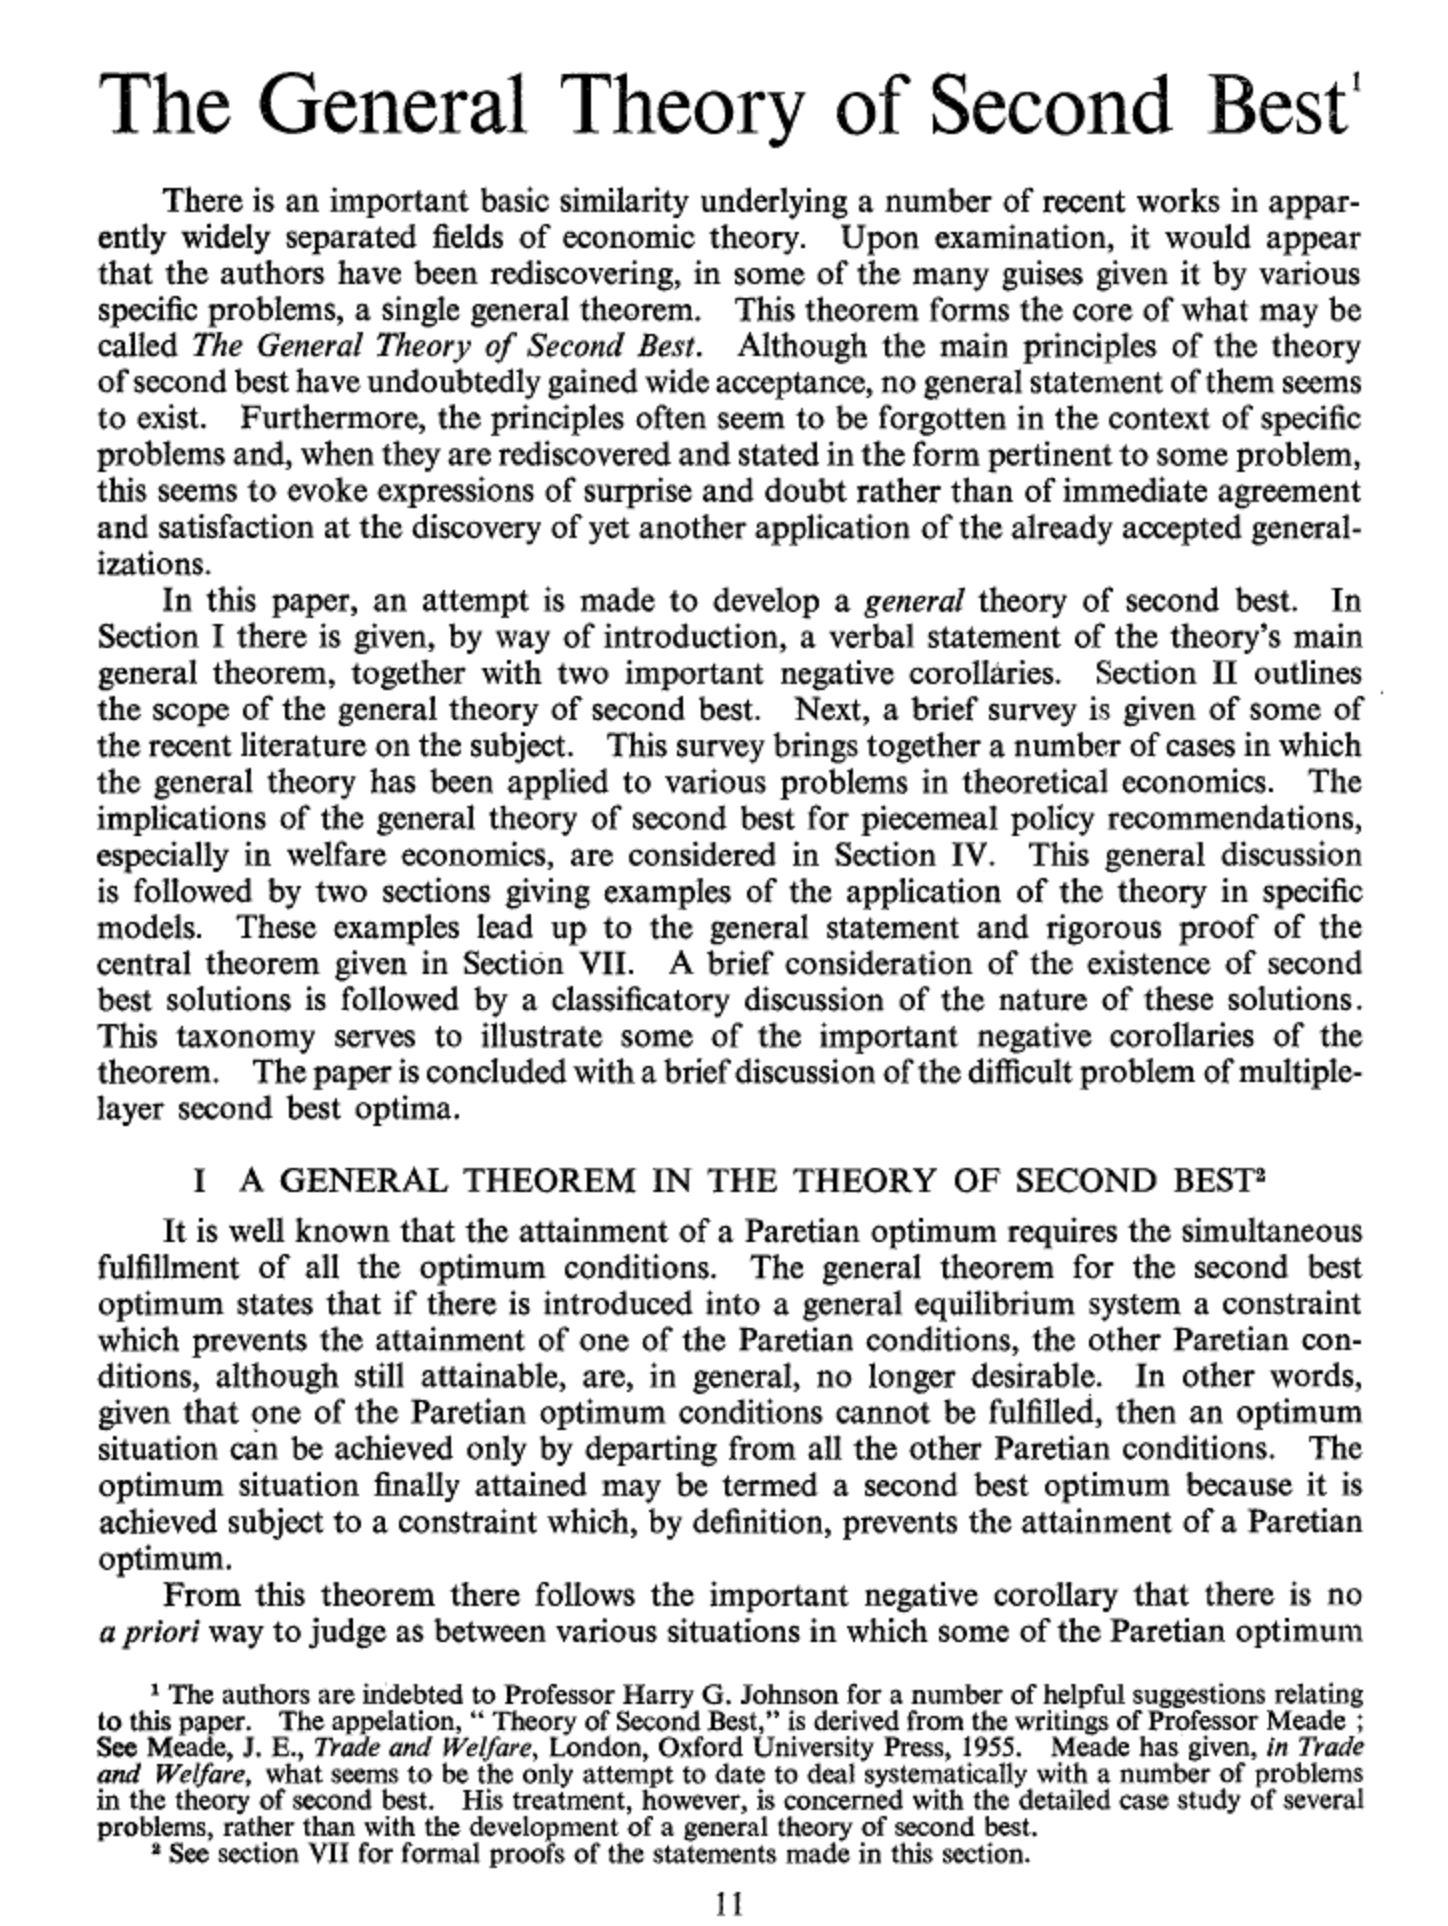
\includegraphics{lipsey.png}

}

\caption{\emph{The General Theory of the Second Best}, by R. G. Lipsey
and Kelvin Lancaster, The Review of Economic Studies, 1956}

\end{figure}%

This is one of the most philosophically important economics papers ever
published.

\subsection{Second Best}\label{second-best}

Often times, the right thing to do is something whose value consists in
mitigating the costs of our other flaws.

\begin{itemize}
\tightlist
\item
  We should, especially in high stakes settings, stop and have a little
  think before acting.
\item
  The ``ideal agent'' of decision theory never stops to have a think.
\item
  Stopping is costly, and \textbf{they} don't gain anything from it.
\end{itemize}

\subsection{Second Best}\label{second-best-1}

\begin{itemize}
\tightlist
\item
  The ideal agent does lots of things we don't do.
\item
  They always take reasonable hedges against costly possibilities, and
  they never stop to have a think.
\item
  Knowing that the ideal agent is \emph{F} doesn't tell us whether we
  should try to be \emph{F} unless we also know that \emph{F} is more
  like the first of these than the second.
\item
  And decision theory, in \textbf{anything like its current form}, is
  not particularly helpful on this score.
\end{itemize}

\subsection{Third Objection - The Yoda
Objection}\label{third-objection---the-yoda-objection}

Decision theory doesn't say what one should try or not try, it says what
one should do.

\begin{itemize}
\tightlist
\item
  So it's weird to infer something about trying from a theory about
  doing.
\end{itemize}

\subsection{Yoda}\label{yoda}

I think there's something importantly right about this - decision theory
gives criteria of correctness not methods of deliberation - but that in
turn shows us why it might be useful.

\section{Idealisations as Models}\label{idealisations-as-models}

\subsection{Two Notions of
Idealisation}\label{two-notions-of-idealisation}

In philosophy we use the word `idealisation' for two rather different
kinds of thing.

\begin{enumerate}
\def\labelenumi{\arabic{enumi}.}
\tightlist
\item
  Perfect
\item
  Simple
\end{enumerate}

The point particles in ideal gas theory are not perfect - having volume
is not an imperfection.

Nor are they things to aim for - high school chemistry does not imply a
rule: \textbf{Smaller the better}.

But they are simple.

\subsection{Idealisations in Decision
Theory}\label{idealisations-in-decision-theory}

Decision theory provides idealisations in the second sense - they are
\textbf{simplifications}.

\begin{itemize}
\tightlist
\item
  Just like the point masses we use in the ideal gas law, they say not
  what should happen, but what would happen in the absence of certain
  complications.
\end{itemize}

\subsection{Idealisations in Decision
Theory}\label{idealisations-in-decision-theory-1}

Why do I say this idealisation is a simplification not a perfection?

\begin{enumerate}
\def\labelenumi{\arabic{enumi}.}
\tightlist
\item
  Allocating zero seconds to hard math problems is not a perfection.
\item
  The idealised self isn't absolutely perfect - they have very
  restricted information.
\end{enumerate}

\subsection{Idealisations in Decision
Theory}\label{idealisations-in-decision-theory-2}

The idealised self that gets used is god-like in one respect -
computational ability - but human-like in another - informational
awareness.

\begin{itemize}
\tightlist
\item
  That's a common feature of idealised models.
\item
  You abstract away from one feature, but not others.
\end{itemize}

\subsection{Why Care?}\label{why-care}

That's what we do, but why do we do it?

\begin{itemize}
\tightlist
\item
  Because sometimes these models are enlightening.
\item
  Sometimes, the fact that we have computational limitations is not
  relevant to predicting/explaining/understanding what we will do.
\end{itemize}

\subsection{Really, Why Care?}\label{really-why-care}

It's tempting to identify these with high stakes situations, since those
are ones where we'll throw enough computational resources at the problem
that we have god-like powers.

\begin{itemize}
\tightlist
\item
  But that isn't quite right.
\item
  In some high stakes cases, we also throw enough investigative
  resources at the problem that holding actual knowledge fixed is a bad
  modeling assumption.
\end{itemize}

\subsection{Informational Limitations}\label{informational-limitations}

What we need are cases where there are principled limitations to our
informational capacities, such as,

\begin{enumerate}
\def\labelenumi{\arabic{enumi}.}
\tightlist
\item
  Cases where the information concerns the future; or
\item
  Cases where someone has (or may have) just as strong an incentive to
  hide information from us.
\end{enumerate}

I'll end with a discussion of an important instance of the
second.\footnote{Photo of George Akerlof on next slide by Yan Chi Vinci
  Chow.}

\subsection{Akerlof on Lemons}\label{akerlof-on-lemons}

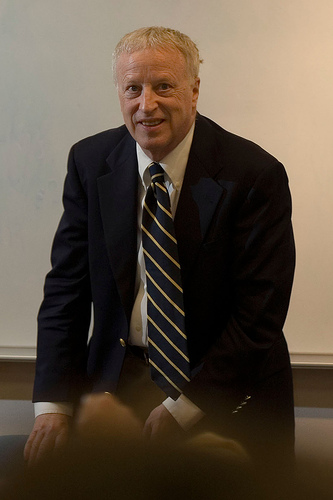
\includegraphics[width=0.8\textwidth,height=0.8\textheight]{akerlof.jpg}


\includegraphics[width=0.71\textwidth,height=0.71\textheight]{lemon.jpg}

\subsection{Akerlof on Lemons}\label{akerlof-on-lemons-1}

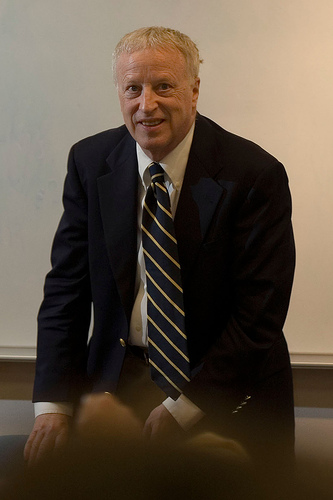
\includegraphics[width=0.8\textwidth,height=0.8\textheight]{akerlof.jpg}

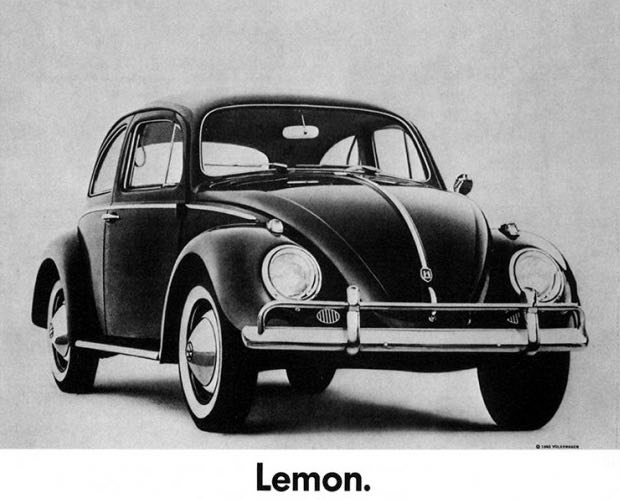
\includegraphics[width=0.8\textwidth,height=0.8\textheight]{vw.jpeg}

\subsection{A 20th Century Puzzle}\label{a-20th-century-puzzle}

Used cars sold at a huge discount to new cars, even when the cars were
just a few months old with almost no usage.

\begin{itemize}
\tightlist
\item
  There was no agreed upon explanation for this, with the most common
  theory being that it reflected a preference/prejudice on the part of
  buyers.
\end{itemize}

\subsection{Akerlof's Theory}\label{akerlofs-theory}

Make the following assumptions.

\begin{enumerate}
\def\labelenumi{\arabic{enumi}.}
\tightlist
\item
  Cars vary a lot in quality, even coming from the same production line.
\item
  Sellers of used cars know how good this token car is.
\item
  Buyers of used cars do not; they only know how good the model is in
  general.
\item
  People rarely sell cars they just bought.
\item
  Everyone involved is an expected utility maximiser.
\end{enumerate}

\subsection{Akerlof's Theory}\label{akerlofs-theory-1}

Akerlof built a formal model with the following properties.

\begin{itemize}
\tightlist
\item
  The most common reason to sell a car one just bought is the discovery
  that it was a bad instance of that kind of car.
\item
  Knowing this, buyers of used cars demanded a big discount in exchange
  for the possibility they were buying a dud.
\item
  Everyone is acting rationally within the model, given their asymmetric
  information.
\end{itemize}

\subsection{Akerlof's Theory}\label{akerlofs-theory-2}

If he was right (and I basically think he was) you'd expect the used car
discount to fall if either of the following things happened.

\begin{enumerate}
\def\labelenumi{\arabic{enumi}.}
\tightlist
\item
  Production lines got more reliable, and cars off the same line were
  more similar to one another; or
\item
  Buyers had access to better tools to judge the quality of used cars.
\end{enumerate}

By 2020 both of those things had happened, and the used car discount was
almost zero. (Then in 2021 it went negative for weird reasons.)

\subsection{Back To Philosophy}\label{back-to-philosophy}

You can't build models like this without a theory of rational action
under uncertainty.

\begin{itemize}
\tightlist
\item
  And that's the payoff of philosophical decision theory.
\item
  It's an essential input to useful models, like this one.
\end{itemize}

\subsection{Consequences for Decision
Theory}\label{consequences-for-decision-theory}

The thing about explanatory models is that they can have very limited
scope.

\begin{itemize}
\tightlist
\item
  There are lots of properties of gases that you cannot explain with the
  ideal gas model.
\end{itemize}

\subsection{Consequences for Decision
Theory}\label{consequences-for-decision-theory-1}

This matters because a lot of people in decision theory assume that a
good decision theory will have something to say about every possible
choice situation.

\begin{itemize}
\tightlist
\item
  But if you're in the business of explanation, it's fine to say that
  the theory only applies in some cases, and it only provides
  explanations in those cases.
\end{itemize}

\subsection{Consequences for Decision
Theory}\label{consequences-for-decision-theory-2}

There are (at least) two interesting notions around here:

\begin{enumerate}
\def\labelenumi{\arabic{enumi}.}
\tightlist
\item
  What the ideal decider would do in a particular situation.
\item
  What it would be advisable for a real life human to do in this
  situation.
\end{enumerate}

\begin{itemize}
\tightlist
\item
  These come apart in Traveling Salesman cases, and we should keep open
  the possibility that they also come apart in cases that philosophers
  talk about.
\end{itemize}

\subsection{For Another Day}\label{for-another-day}

At this point you might expect that I'd have a theory that does go
silent on a bunch of hard cases, and which explains away a bunch of
intuitions about cases as intuitions about advisability, not about what
an ideal decider does, and you'd be right on both counts.

\begin{itemize}
\tightlist
\item
  And I'm happy to talk about that theory (and those cases) at literally
  any length people want.
\item
  But it's mostly for another talk.
\end{itemize}

\subsection{For Yet Another Day}\label{for-yet-another-day}

You might also wonder at this point whether there are other
idealisations we could make, which are useful in different circumstances
to the standard computationally perfect, informationally limited model.

\begin{itemize}
\tightlist
\item
  I used to think the answer was no on broadly a priori grounds.
\item
  But this was wrong, and the work on cursed equilibrium shows it was
  wrong.
\item
  There are some potentially really interesting questions here for
  philosophy of economics that engages seriously with 21st century
  economics.
\end{itemize}

\subsection{Conclusions}\label{conclusions}

\begin{itemize}
\tightlist
\item
  Decision theory provides idealisations.
\item
  These are not things we should aim for, but simplifications that play
  a role in explanations.
\end{itemize}



\end{document}
